\section{Application of probabilistic catalogs for population studies}
\lb{sec:dNdS}



\begin{figure*}[h]
\center
%\hspace*{-1cm}
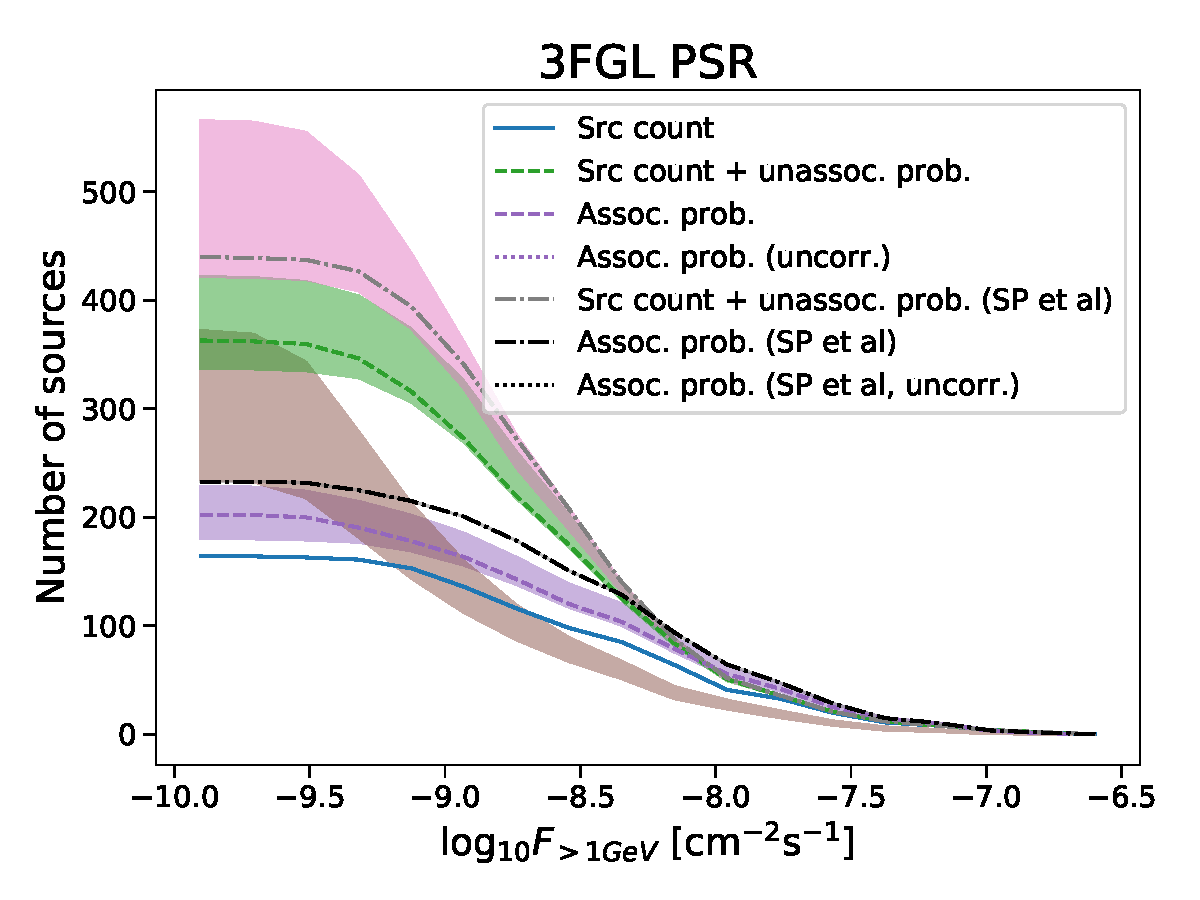
\includegraphics[width=0.42\textwidth]{plots/N_logS_3FGL_PSR_SazP.pdf}
%\hspace*{-1cm}
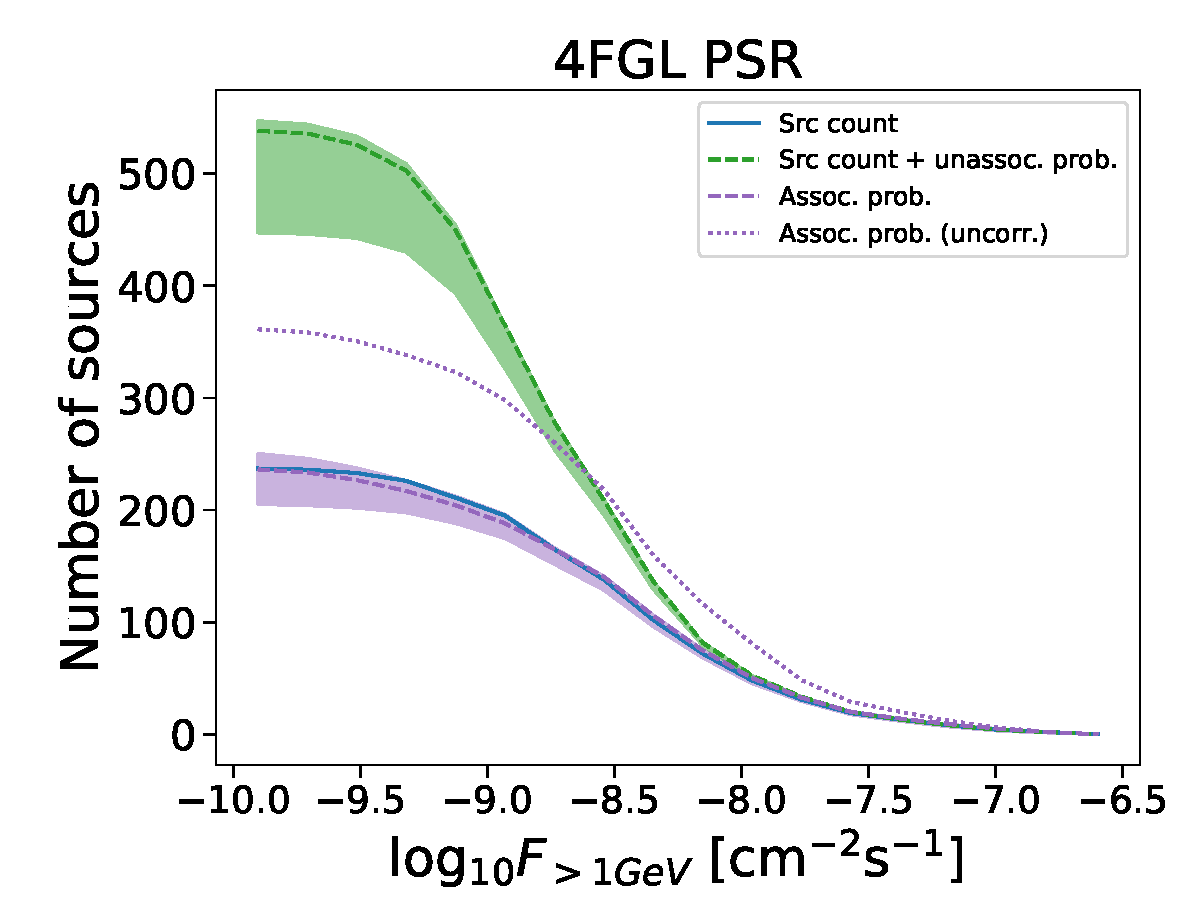
\includegraphics[width=0.42\textwidth]{plots/N_logS_4FGL_PSR.pdf} \\
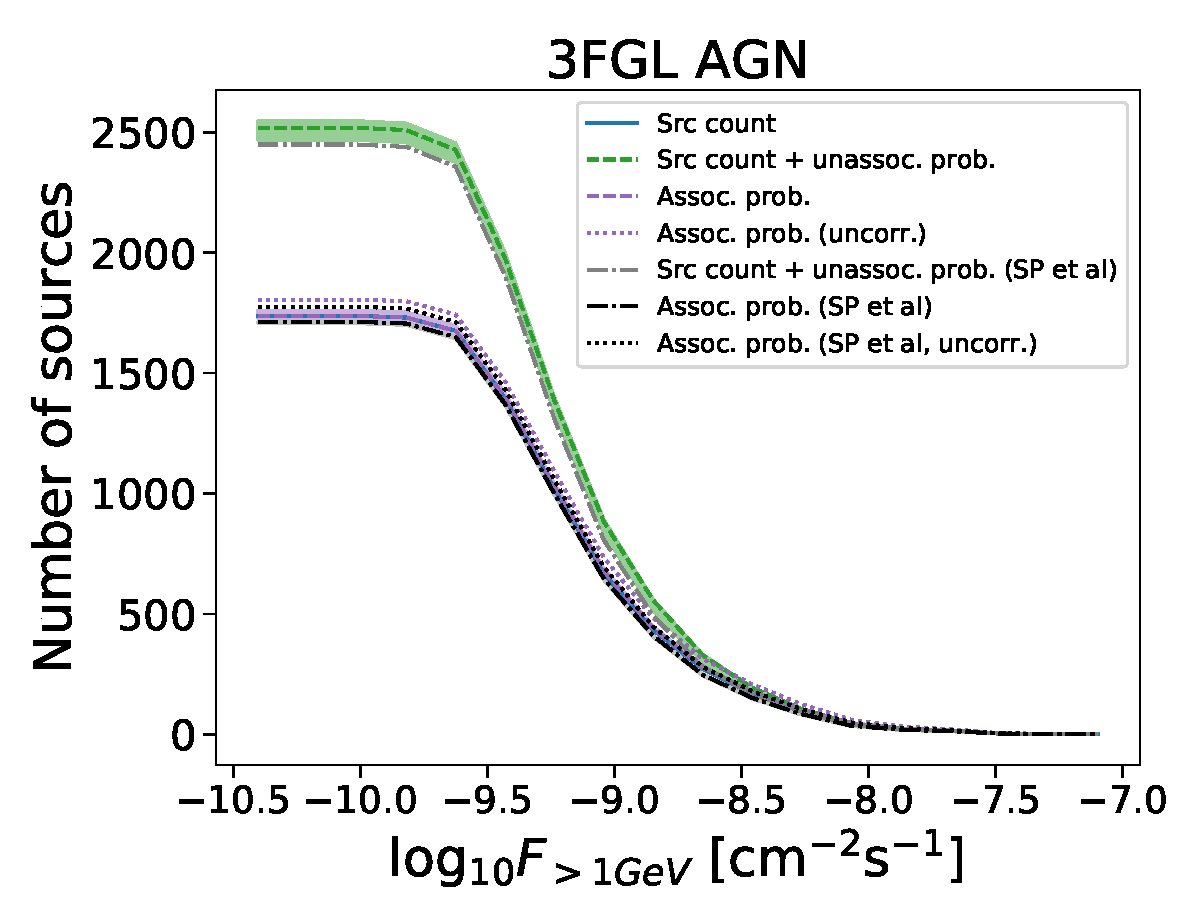
\includegraphics[width=0.42\textwidth]{plots/N_logS_3FGL_AGN_SazP.pdf}
%\hspace*{-1cm}
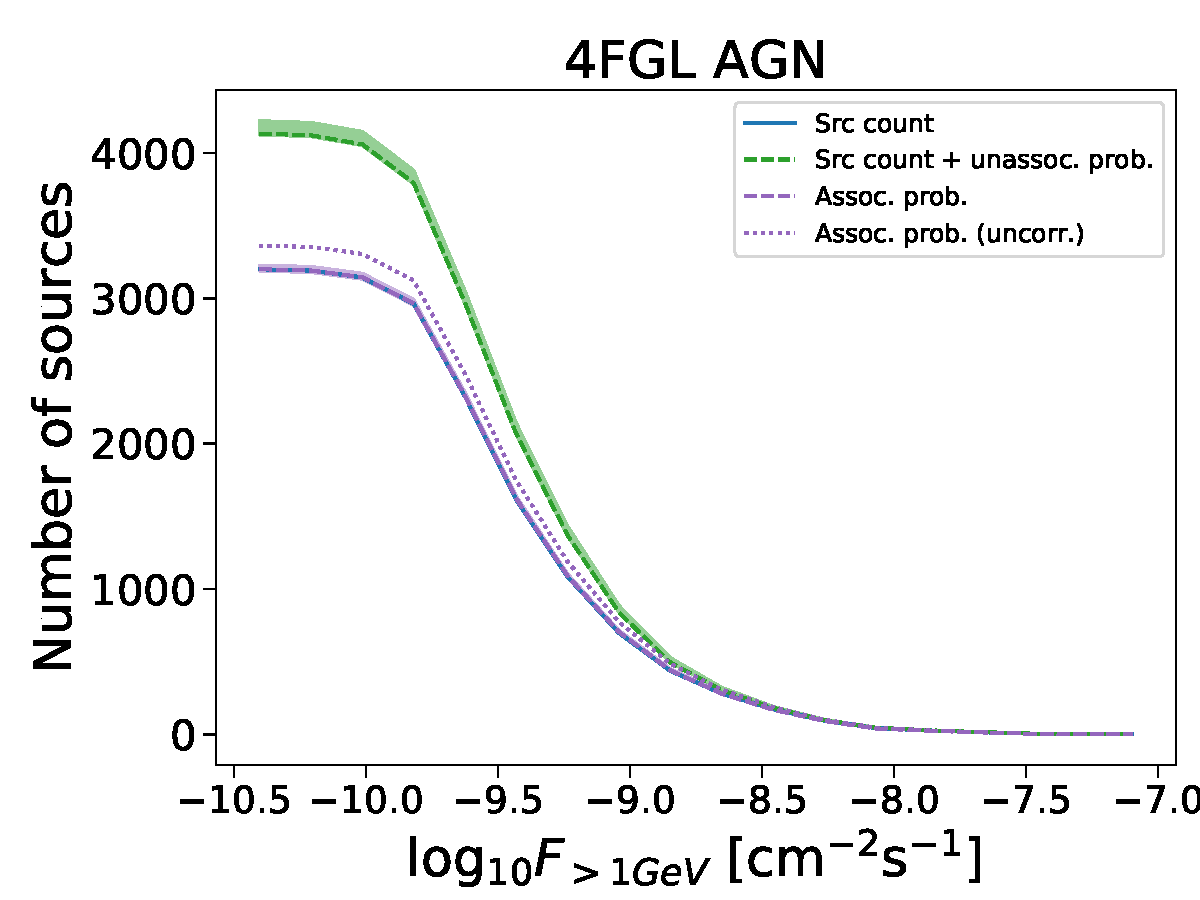
\includegraphics[width=0.42\textwidth]{plots/N_logS_4FGL_AGN.pdf}
\caption{Cumulative number of sources as a function of their flux.}  
\label{fig:logN_logS}
\end{figure*}


\begin{figure}[h]
\center
%\hspace*{-1cm}
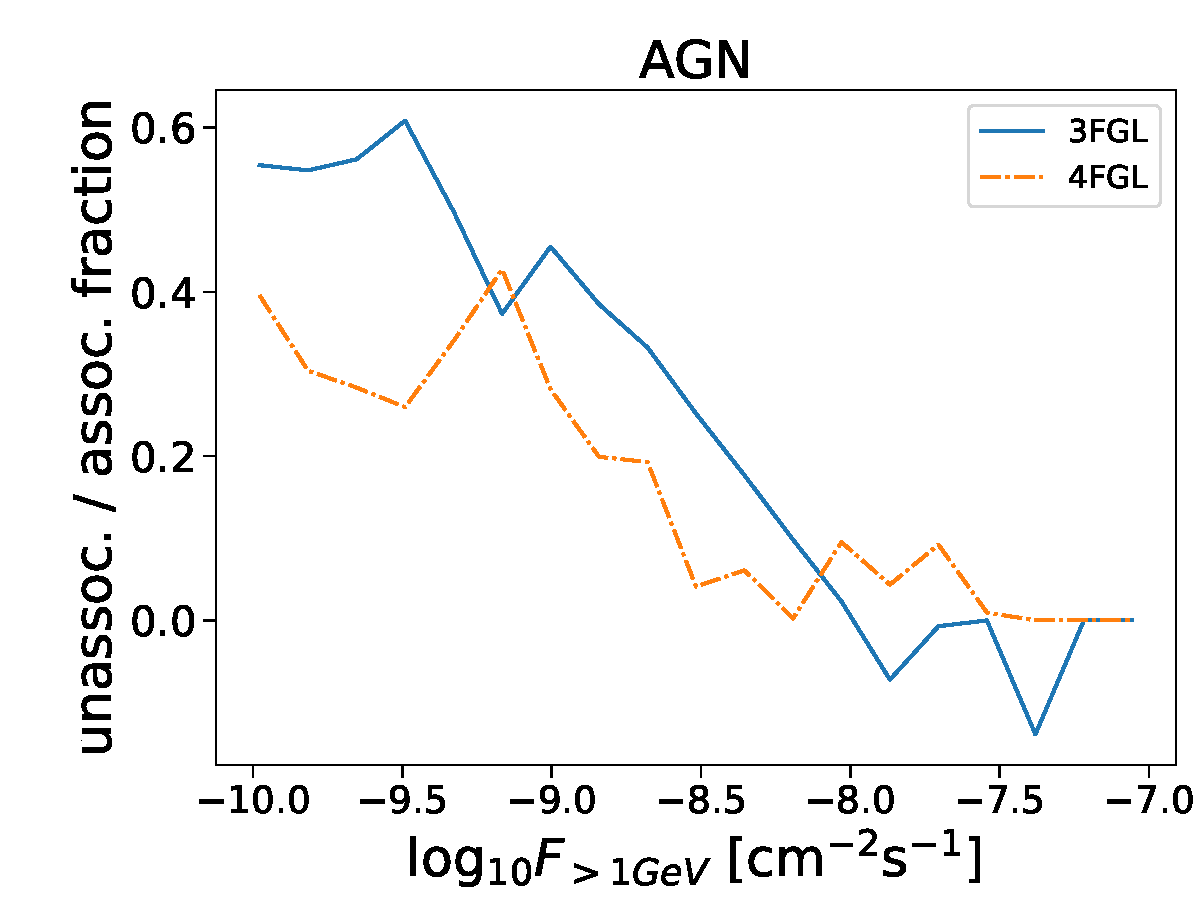
\includegraphics[width=0.42\textwidth]{plots/logN_logS_diff_AGN_unweighted.pdf}
%\hspace*{-1cm}
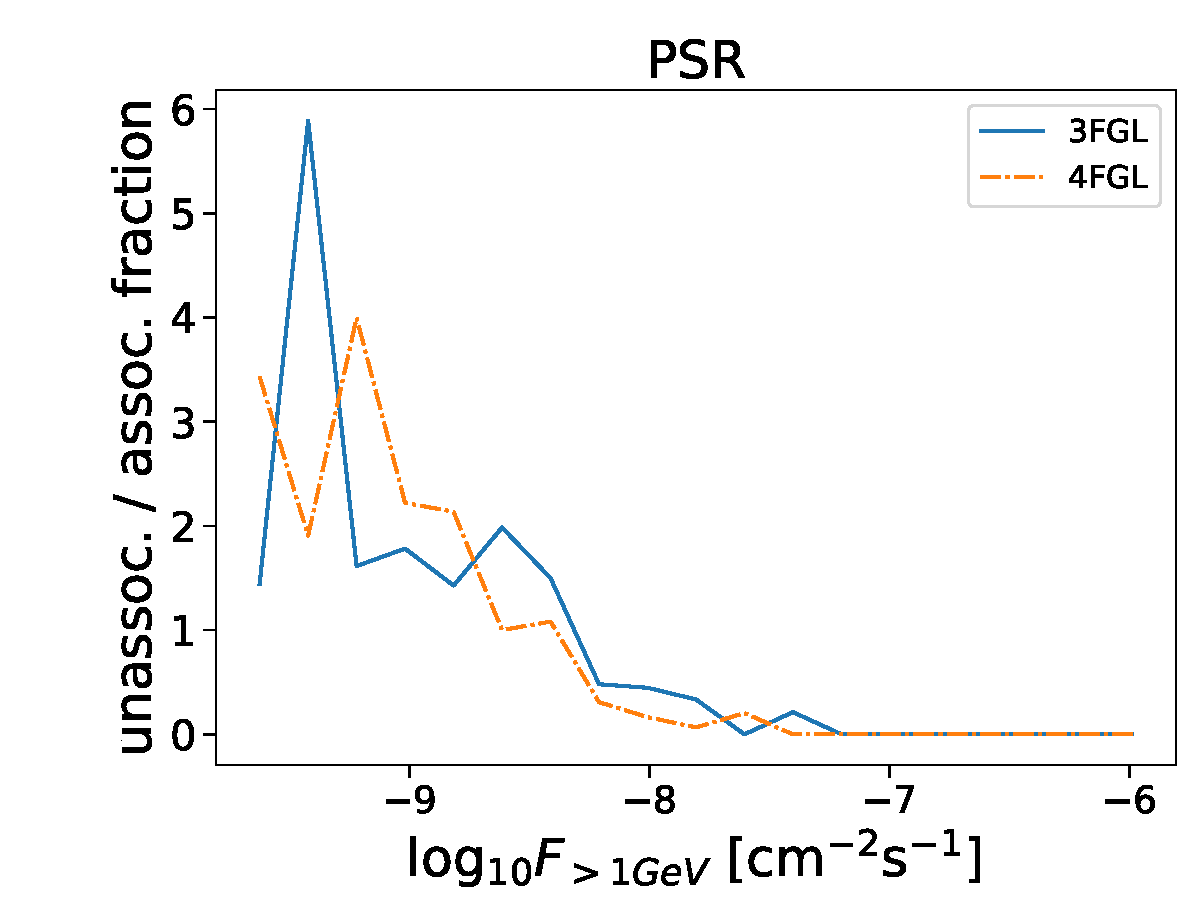
\includegraphics[width=0.42\textwidth]{plots/logN_logS_diff_PSR_unweighted.pdf}
\caption{Fraction of unassociated sources relative to associated ones.}  
\label{fig:unass_vs_ass_frac}
\end{figure}



In this section we show how probabilistic catalogs can be used, for instance, for population studies.
One of the most important questions in gamma-ray astronomy is contribution of point sources, e.g., AGNs, to the extragalactic gamma-ray
flux:
if most of the extra-galactic emission is explained by point sources, then one can put stringent constraints, e.g., on 
dark matter annihilation into gamma rays, on evaporation of primordial black holes, and on the origin of astrophysical high energy neutrino flux.
In particular, it is important to understand the contribution to the population of AGNs from the unassociated sources.
A probabilistic catalog provides an answer to the question: how many sources among the unassociated ones are expected to belong to different classes, such as pulsars or AGNs. 
One can calculate the total expected number of AGNs or pulsars among the unassociated sources, or calculate the contribution as a function of one or more parameters.
In this section we determine the numbers of AGNs and pulsars as a function of their flux.

In Figure \ref{fig:logN_logS} we show the cumulative number of AGNs and pulsars with flux above 1 GeV larger than the
value on the x-axis.
Solid lines show the actual counts of sources (AGNs or pulsars) in the 3FGL and 4FGL catalogs.
As a consistency check of the method, we calculate the AGN- and PSR-like probabilities for associated sources.
The sum of probabilities (uncorrected for sources other than AGNs and pulsars) for LR algorithm are shown by dotted purple lines.
In order to correct the expected number of AGNs among associated sources for AGN-like probabilities in ``other'' sources, 
we subtract the corresponding AGN-like probabilities in each flux band:

\be
\lb{eq:assoc_ev}
N_{\rm AGN}^{\rm ass}  = \sum_{i \in \rm ass} p^i_{\rm AGN}\,\, - \sum_{i \in \rm ass\,other} p^i_{\rm AGN}.
\ee
The corrected sums of probabilities for LR method are shown by dashed purple lines.
The purple bands show the envelope of the sum of corrected probabilities for the four methods used in this paper.
We see that the counts of associated sources, AGNs and pulsars, are consistent with the expected number of associated sources
calculated from the class probabilities of associated sources.
This conclusion is not very surprising since we used associated sources for training of ML algorithms.
It is important to note that correction for ``other'' sources is important for consistency of the sum of probabilities and the number of associated sources.
We have also compared the sums of probabilities for the 3FGL associated sources in \cite{2016ApJ...820....8S}.%
\footnote{The data is downloaded from \url{https://www.physics.hku.hk/~pablo/pulsarness.html}.}
The sum of probabilities for associated sources in the LR case uncorrected for ``other'' sources are shown by dotted black line,
while the sums corrected for ``other'' sources are shown by black dash-dotted lines.
The gray band is the envelope of the two methods (LR and RF) used by \cite{2016ApJ...820....8S}.
We see that the sum of probabilities for pulsars overpredicts the pulsar counts in 3FGL, correction for ``other'' sources makes the prediction 
more consistent with the counts of pulsars, although it is still overpredicting them.

We note that the expected number of associated pulsars in 3FGL and 4FGL catalogs (purple band) is slightly below the 
actual counts of pulsars, this can be due to the fact that the number of AGNs in the training sample is much larger than the number of pulsars.
\cite{2016ApJ...820....8S} have used weights in the training sample inversely proportional to the number of elements in the class,
i.e., a pulsar has more weight in training than an AGN.
This can be a reason for an overprediction of the number of associated pulsars, compared to the actual count.


The predictions for the number of AGNs and pulsars among the unassociated sources corrected for ``other'' sources 
added to the 3FGL and 4FGL source counts are shown by green dashed lines (for the LR case).
The green bands show the corresponding envelopes for the four ML algorithms.
We assume that the fractional contribution of other sources is the same for associated and unassociated sources in the different flux bands.
Thus, the correction for the presence of other sources is calculated similarly to the associated sources in Equation \ref{eq:assoc_ev},
but we adjust for the fact that there are fewer unassociated than associated sources, i.e., 
the correction is assumed to be proportionally smaller.
In particular, the number of AGNs among unassociated sources in a certain flux band $\Delta F$ is estimated as

\be
\lb{eq:unassoc_ev}
N_{\rm AGN}^{\rm unass} = \sum_{i \in \rm unass} p^i_{\rm AGN}\,\, - \sum_{i \in \rm ass\,other} p^i_{\rm AGN} \cdot 
\frac{N_{\rm unass}}{N_{\rm ass}}
\ee
where all probabilities and the numbers of sources are computed for sources with flux inside $\Delta F$.
The first term is the sum of AGN-like probabilities among the unassociated sources,
while the second term is the sum of AGN-like probabilities among associated ``other'' sources rescaled by the total number
of unassociated and associated sources in this flux band.
The expected number of pulsars among the unassociated sources is calculated analogously.
A few conclusions based on Figure \ref{fig:logN_logS} are in order:
\ben
\item
The total number of AGNs among the detected 3FGL or 4FGL sources is about 50\% higher than the number of associated AGNs.
This conclusion is not very surprising since the number of unassociated sources is about 1/3 of the total number of sources and the 
AGNs are the largest class of sources. It is important to note, however, that the different ML algorithms provide a reasonable uncertainty band on the number of AGNs among the unassociated sources, which is, in particular, smaller than the expected number of pulsars among the unassociated sources.
\item
The number of pulsars among the unassociated sources is about the same as the number of associated pulsars, i.e., the total number of pulsars among the detected sources is expected to be twice the number of associated pulsars.
\een
We predict that the expected number of pulsars among the unassociated sources in the 3FGL catalog
is $200 \pm 40$, where the range is the envelop of the sums of probabilities in Equation (\ref{eq:unassoc_ev})
for different ML methods corrected for other sources among the unassociated sources.
The expected number of pulsars among the unassociated sources in the 4FGL catalog corrected for other sources is $260 \pm 50$.
We note that according to Table \ref{tab:3FGL_prediction}, the number of unassociated 3FGL sources 
with $p_{\rm PSR} > 0.5$ for all four ML algorithms is 97 (81.5), while there are 182 (164.5) sources with mixed classification,
uncorrected (corrected) for other sources.
The number of pulsars with mixed classification (164.5 for 3FGL or 221.3 for 4FGL)
is about two times larger than the range of values for the expected number of pulsars calculated for the sum of probabilities 
(80 for 3FGL or 100 for 4FGL).
It means that the decision which sources are considered to be more likely pulsars is more sensitive to the choice of the ML method
and the probability threshold than the expected number of pulsars (based on the sum of probabilities).

We also note that the probabilistic classification mostly affects sources with smaller fluxes,
which we illustrate in Figure \ref{fig:unass_vs_ass_frac}, where we show that the ratio of expected number of AGNs and pulsars among unassociated sources computed according to Equation \ref{eq:unassoc_ev} to the number of associated sources decreases as the flux increases.
Negative values (e.g., at high fluxes for AGNs) are due to subtraction of probabilities for the ``other'' associated sources.
%One can see that the fraction of AGNs or pulsars among unassociated sources to the associated ones is higher at smaller fluxes.






